\documentclass[tikz,border=2pt]{standalone}
\usepackage{pgfplots}
\usepgfplotslibrary{groupplots}
\pgfplotsset{compat=1.18}

\begin{document}
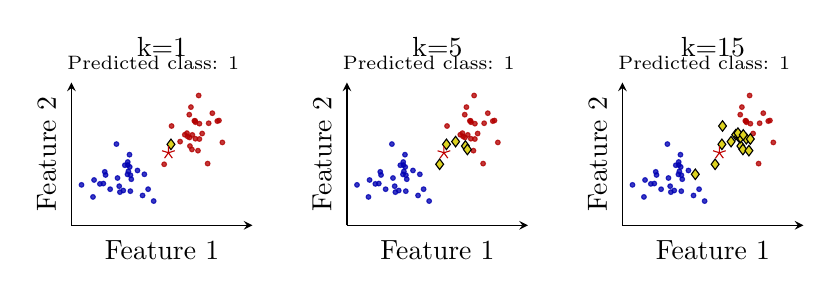
\begin{tikzpicture}
\begin{groupplot}[
  group style={group size=3 by 1, horizontal sep=1.2cm},
]

\nextgroupplot[
  title={k=1},
  xmin=-3.5,xmax=3.5,
  ymin=-3.2,ymax=3.2,
  axis lines=left,
  xlabel={Feature 1}, ylabel={Feature 2},
  tick style={draw=none},
  xtick=\empty, ytick=\empty,
  width=0.32\textwidth,
  height=0.28\textwidth,
  clip=false,
]
\addplot[only marks, mark=*, mark size=0.85pt, draw=blue!70!black, fill=blue!70!black, opacity=0.78] coordinates {(-1.29911,-0.78490) (-1.49738,-1.64123) (-1.62736,-1.71399) (-1.25670,-0.03505) (-1.65439,-1.44674) (-0.94731,-0.74304) (-1.22410,-1.66994) (-1.32106,-0.49938) (-2.26783,-1.32948) (-2.66888,-1.92847) (-2.62605,-1.16927) (-2.21256,-0.80469) (-1.18714,-1.13459) (-3.11207,-1.38786) (-1.33492,-0.91842) (-2.40170,-1.34398) (-2.00453,-1.58236) (-0.53615,-1.58142) (-1.32342,-0.36324) (-1.72019,-1.08043) (-1.22047,-0.95408) (-2.18204,-0.94518) (-0.32165,-2.11394) (-0.68124,-0.91407) (-1.76186,0.44030) (-0.75117,-1.86349) (-1.24635,-0.58478) (-1.43592,-0.50830)};
\addplot[only marks, mark=*, mark size=0.85pt, draw=red!70!black, fill=red!70!black, opacity=0.78] coordinates {(1.25211,1.48042) (2.33574,0.51352) (1.44626,0.66642) (1.39163,0.14522) (0.88290,0.85874) (1.94711,1.82456) (0.34706,0.42786) (1.76577,-0.43454) (0.96652,0.92995) (2.20505,1.49637) (1.06441,0.73463) (1.11986,2.09694) (0.99182,0.78135) (1.55386,0.91305) (1.15796,0.19787) (1.29170,0.68062) (2.13961,1.47022) (1.28262,1.48123) (1.05529,1.75753) (1.29611,1.42004) (0.37056,1.24961) (0.08449,-0.46544) (1.08078,0.35205) (1.41812,2.61622) (0.70116,0.55076) (1.44789,1.35497) (1.17299,0.85173) (1.80577,1.37433)};
\addplot[only marks, mark=diamond*, mark size=1.9pt, draw=black, fill=yellow!85!black] coordinates {(0.34706,0.42786)};
\addplot[only marks, mark=star, mark size=2.4pt, draw=red!75!black, fill=red!75!black] coordinates {(0.25000,0.05000)};
\node[anchor=south east, font=\scriptsize] at (rel axis cs:0.98,1.02) {Predicted class: 1};

\nextgroupplot[
  title={k=5},
  xmin=-3.5,xmax=3.5,
  ymin=-3.2,ymax=3.2,
  axis lines=left,
  xlabel={Feature 1}, ylabel={Feature 2},
  tick style={draw=none},
  xtick=\empty, ytick=\empty,
  width=0.32\textwidth,
  height=0.28\textwidth,
  clip=false,
]
\addplot[only marks, mark=*, mark size=0.85pt, draw=blue!70!black, fill=blue!70!black, opacity=0.78] coordinates {(-1.29911,-0.78490) (-1.49738,-1.64123) (-1.62736,-1.71399) (-1.25670,-0.03505) (-1.65439,-1.44674) (-0.94731,-0.74304) (-1.22410,-1.66994) (-1.32106,-0.49938) (-2.26783,-1.32948) (-2.66888,-1.92847) (-2.62605,-1.16927) (-2.21256,-0.80469) (-1.18714,-1.13459) (-3.11207,-1.38786) (-1.33492,-0.91842) (-2.40170,-1.34398) (-2.00453,-1.58236) (-0.53615,-1.58142) (-1.32342,-0.36324) (-1.72019,-1.08043) (-1.22047,-0.95408) (-2.18204,-0.94518) (-0.32165,-2.11394) (-0.68124,-0.91407) (-1.76186,0.44030) (-0.75117,-1.86349) (-1.24635,-0.58478) (-1.43592,-0.50830)};
\addplot[only marks, mark=*, mark size=0.85pt, draw=red!70!black, fill=red!70!black, opacity=0.78] coordinates {(1.25211,1.48042) (2.33574,0.51352) (1.44626,0.66642) (1.39163,0.14522) (0.88290,0.85874) (1.94711,1.82456) (0.34706,0.42786) (1.76577,-0.43454) (0.96652,0.92995) (2.20505,1.49637) (1.06441,0.73463) (1.11986,2.09694) (0.99182,0.78135) (1.55386,0.91305) (1.15796,0.19787) (1.29170,0.68062) (2.13961,1.47022) (1.28262,1.48123) (1.05529,1.75753) (1.29611,1.42004) (0.37056,1.24961) (0.08449,-0.46544) (1.08078,0.35205) (1.41812,2.61622) (0.70116,0.55076) (1.44789,1.35497) (1.17299,0.85173) (1.80577,1.37433)};
\addplot[only marks, mark=diamond*, mark size=1.9pt, draw=black, fill=yellow!85!black] coordinates {(0.34706,0.42786) (0.08449,-0.46544) (0.70116,0.55076) (1.08078,0.35205) (1.15796,0.19787)};
\addplot[only marks, mark=star, mark size=2.4pt, draw=red!75!black, fill=red!75!black] coordinates {(0.25000,0.05000)};
\node[anchor=south east, font=\scriptsize] at (rel axis cs:0.98,1.02) {Predicted class: 1};

\nextgroupplot[
  title={k=15},
  xmin=-3.5,xmax=3.5,
  ymin=-3.2,ymax=3.2,
  axis lines=left,
  xlabel={Feature 1}, ylabel={Feature 2},
  tick style={draw=none},
  xtick=\empty, ytick=\empty,
  width=0.32\textwidth,
  height=0.28\textwidth,
  clip=false,
]
\addplot[only marks, mark=*, mark size=0.85pt, draw=blue!70!black, fill=blue!70!black, opacity=0.78] coordinates {(-1.29911,-0.78490) (-1.49738,-1.64123) (-1.62736,-1.71399) (-1.25670,-0.03505) (-1.65439,-1.44674) (-0.94731,-0.74304) (-1.22410,-1.66994) (-1.32106,-0.49938) (-2.26783,-1.32948) (-2.66888,-1.92847) (-2.62605,-1.16927) (-2.21256,-0.80469) (-1.18714,-1.13459) (-3.11207,-1.38786) (-1.33492,-0.91842) (-2.40170,-1.34398) (-2.00453,-1.58236) (-0.53615,-1.58142) (-1.32342,-0.36324) (-1.72019,-1.08043) (-1.22047,-0.95408) (-2.18204,-0.94518) (-0.32165,-2.11394) (-0.68124,-0.91407) (-1.76186,0.44030) (-0.75117,-1.86349) (-1.24635,-0.58478) (-1.43592,-0.50830)};
\addplot[only marks, mark=*, mark size=0.85pt, draw=red!70!black, fill=red!70!black, opacity=0.78] coordinates {(1.25211,1.48042) (2.33574,0.51352) (1.44626,0.66642) (1.39163,0.14522) (0.88290,0.85874) (1.94711,1.82456) (0.34706,0.42786) (1.76577,-0.43454) (0.96652,0.92995) (2.20505,1.49637) (1.06441,0.73463) (1.11986,2.09694) (0.99182,0.78135) (1.55386,0.91305) (1.15796,0.19787) (1.29170,0.68062) (2.13961,1.47022) (1.28262,1.48123) (1.05529,1.75753) (1.29611,1.42004) (0.37056,1.24961) (0.08449,-0.46544) (1.08078,0.35205) (1.41812,2.61622) (0.70116,0.55076) (1.44789,1.35497) (1.17299,0.85173) (1.80577,1.37433)};
\addplot[only marks, mark=diamond*, mark size=1.9pt, draw=black, fill=yellow!85!black] coordinates {(0.34706,0.42786) (0.08449,-0.46544) (0.70116,0.55076) (1.08078,0.35205) (1.15796,0.19787) (0.88290,0.85874) (0.99182,0.78135) (1.06441,0.73463) (0.96652,0.92995) (1.39163,0.14522) (0.37056,1.24961) (1.29170,0.68062) (1.17299,0.85173) (-0.68124,-0.91407) (1.44626,0.66642)};
\addplot[only marks, mark=star, mark size=2.4pt, draw=red!75!black, fill=red!75!black] coordinates {(0.25000,0.05000)};
\node[anchor=south east, font=\scriptsize] at (rel axis cs:0.98,1.02) {Predicted class: 1};

\end{groupplot}
\end{tikzpicture}
\end{document}
